\chapter{Developing the Hardware} % Main chapter title

\label{Chapter4} % Change X to a consecutive number; for referencing this chapter elsewhere, use \ref{ChapterX}


\section{Requirements}\label{sec:HardwareRequirements}

This section will explain the different constraints taken into account while developing the hardware portion of this project.
First, the hardware must be performant enough to provide a positive user experience (\ref{sec:HardwarePerformance}), and secondly the product must be cheap enough to justify it over similar alternatives (\ref{sec:HardwareCost}).

\subsection{Performance}\label{sec:HardwarePerformance}

When considering how much power needs to be incorporated in to the miniature computer, it is important to consider a number of factors, such as: having enough power to stream audio and video over the internet, not consuming too much power so as to require an expensive battery, have a fast enough connection to the internet to deliver data with the least possible latency, and having a reasonable footprint to be used as a mobile device.

Immediately, the device must be capable of decoding and rendering video that is streamed over the internet; a relatively expensive process that cannot easily be done with something such as a micro controller or even a single core CPU seen on Single Board Computers (SBC) such as the \todo{pic?}Raspberry Pi Zero.
Though at the same time, it is important to not simply build a powerful system akin to a laptop that will consume more power.
It makes no sense to built a powerful mini-computer when all it will ever be used to is to connect to another computer, and the added power draw would require a larger battery in order to stay operational for decent periods of time.
Instead it should be cut down and distilled into something that can do it's job as efficiently as possible.

The second major performance requirement of the hardware is the ability to stream this data over the internet as quickly as possible.
Because all of the data being sent to the device is live information from the host machine, the video and audio streams cannot simply be buffered in advance and played when it's ready like a recorded video.
Instead, the data must be displayed as it is received so that the user can have a smooth experience without having to wait for their keystrokes or mouse movements to be registered.
While Wi-Fi is growing ever quicker and more reliable, and should absolutely be included as a way to connected to the internet, the best way to ensure a stable and speedy connection is to use an Ethernet Cable.
This will help the device work on a consistent connection when used at a desk, while also providing a way to connect while on-the-go.

This leads to the desire for a portable design that can be used both in a conducive environnement such as a desk or while mobile.
The hardware should have the ability to be powered by a chord plugging into the device, or by an internal battery.
This alone presents a number of difficult concerns, but those will be addressed later in this chapter\todo{cite}.
Such a requirement leads to a clear benefit of integrating crucial computers such as a battery and a screen into the hardware design, while leaving as many ports open such as ethernet and USB for the user to take advantage of.


\subsection{Cost}\label{sec:HardwareCost}

Because this project consists of both a Hardware and Software component to make up a complete product, there must be reason for both to exist.
While the software has the benefit of being the foundation for the connection between host and client machines, there are already hardware solutions that would theoretically be able to run such software.
Since the goal of this project is to save money by not needing to purchase an expensive mobile device to connect to a powerful desktop computer, there must be benefit in the hardware to warrant it's existence over repurposing something like an old laptop.
The most obvious metric of this is the actual cost of the hardware.
If the hardware can be produced at a high enough quality at a low enough cost to bring value over just a software solution, then it should be considered moving forward.
Otherwise it may prove that the development of the software should focus on compatibility so the hardware can be provided by the end user.


\section{Choosing Parts}\label{sec:ChoosingParts}

When starting to choose parts for the hardware, \todo{First person, now this is me explaining what I did?}I had many difficult questions to face.
First and foremost, as a Software Engineer with no experience with Electrical Engineering, I had to make sure I could build the hardware in a way that I could handle.
Specifically, I knew I shouldn't even attempt to build a Single Board Computer on my own, but I knew I also did not want to purchase an off the shelf SBC that was not tailored to the task at hand such as a traditional Raspberry Pi.
Instead I opted for a \emph{Raspberry Pi Compute Module 4 (CM4)} which has \enquote{The power of Raspberry Pi 4 in a compact form factor for deeply embedded applications} \cite{rpi_cm4}.
Boasting an incredibly small size and streamlined I/O, there only way to communicate with the Compute Module was through two tiny mezzanine connectors as shown in Figure \ref{fig:rpi_cm4_mezzanine}.
With no other pin outs for anything such as power, HDMI, or USB, everything had to be built on a custom Printed Circuit Board (PCB).

\begin{figure}[h]
  \centering
  \begin{minipage}{0.45\textwidth}
    \centering
    \includegraphics[width=0.9\textwidth]{Figures/rpi_cm4}
    \captionsetup{width=.75\linewidth}
    \caption[Raspberry Pi Compute Module 4]{Raspberry Pi Compute Module 4, sizing\newline55 x 40mm}
    \label{fig:rpi_cm4}
  \end{minipage}\hfill
  \begin{minipage}{0.45\textwidth}
    \centering
    \includegraphics[width=0.9\textwidth]{Figures/rpi_cm4_mezzanine}
    \captionsetup{width=.75\linewidth}
    \caption[Raspberry Pi Compute Module 4 Pin out]{Close-up of the pin out, with a 0.04mm pitch between pins}
    \label{fig:rpi_cm4_mezzanine}
  \end{minipage}
\end{figure}

This PCB would have to be designed so that the CM4 could be plugged into the board using the mezzanine connectors and rely on it for all inputs and outputs.
This, however, is only the beginning of the story.
Since I would not be working with an off the shelf SBC like a regular Raspberry PI, I would have to not only design the PCB but also pick out all the components that would go onto the PCB, such as the USB ports themselves, the USB driver chip, and related components needed for operation.
Because the CM4 is designed to be as low-powered and compact as possible, some features that would usually be expected of such a device, like the USB ports, are disabled by default and must instead be built by the board designer.
While this helps greatly by removing extraneous components and features that aren't needed for this project, it also provides me with a \todo{does this sound sarcastic?}great opportunity to learn exactly what parts are being used in the hardware.

An invaluable resource while designing the PCB was the Official I/O board for the CM4 \cite{rpi_cm4_io}.
Though I'd still have to build my PCB board on my own and replace components due to the ongoing chip shortage, I wouldn't need to start from scratch.
Another massive benefit from working within the Raspberry Pi Ecosystem is their \todo{(re)move?}incredible documentation and community surrounding the boards.
Around the time I was starting this project, the CM4 was just starting to get into the hands of makers and developers, and only a couple custom boards had actually been made by anyone other than Raspberry Pi themselves.
Even though this leaves the community with less of a bulk of knowledge to work with, it has provided a sort of comradery with everyone helping each other learn the new Compute Module together.
Members of the CM4 engineering team would even assist those on the forums to help them pick parts and design their own boards.


\section{Prototyping}\label{sec:Prototyping}

Whenever working with electrical projects such as this, it is always a good idea to build up prototypes before committing to a final design that will be produced at the highest quality.
I have had experience with building breadboards and even some breakout boards for some components on other projects in the past, but due to the nature of the complex Surface Mounted Devices (SMD) required for this project as well as the dependence on the CM4's tiny mezzanine connectors, building a prototype using a breadboard is infeasible for the amount of time and resources at my disposal.
For example, the USB controller's footprint packs 64 pins into as small of a package as possible, requiring a breakout board of considerable size in order to access each pin separately by hand in a way that could be easily prototyped with.
Not to mention the difficulty in wiring up that many pins along with the other related components which would need their own breakout boards either purchased or custom-designed.

\begin{figure}[h]
  \centering
  %Height instead of width because the image is rotated
  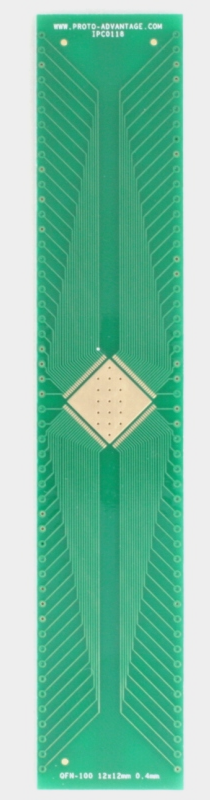
\includegraphics[height=0.9\textwidth,angle=90]{Figures/smt_breakout}
  \captionsetup{width=.8\linewidth}
  \caption[SMD Breakout Board]{A breakout board similar to what would be needer for the USB controller used on the custom PCB}
  \label{fig:smt_breakout}
\end{figure}

Instead, I opted to build out my first board in a piecewise fashion, allowing each section of the board a way to fail without interrupting the rest of the board.
This allows me to test each function of the board individually and in isolation so that changes could be made incrementally without needing to worry about their integration with the rest of the board.
For example, in order to build a system that would allow the board to be powered via USB or an internal battery, as well as charge the battery simultaneously, I would need to build a complex circuit consisting of parts neither I nor anyone I knew had used before.
Since power is obviously a critical component of the board, I would also need to build a secondary way of feeding power directly the board to bypass all that circuitry in case it fails.
In doing so, I can still power the board and test it's other features while developing a fix for that portion of the circuitry for the next iteration.


\section{Designing the Printed Circuit Board}\label{sec:DesigningThePCB}

\todosection


\section{Manufacturing the Circuit Board}\label{sec:ManufacturingThePCB}

\todosection